% =========================  导言区  =========================
\documentclass{beamer}

\usetheme{metropolis}
\usecolortheme[style=light]{Nord}
\usefonttheme[onlymath]{serif}
\metroset{
    numbering = fraction,
    sectionpage = progressbar,
    progressbar = frametitle
}

\usepackage[UTF8]{ctex}

\usepackage{datetime2}

\usepackage{amsmath}
\usepackage{amssymb}
\usepackage{bm}
\usepackage{newtxmath}
\usepackage{cancel}

\usepackage{siunitx}
\usepackage{tabularx}
\usepackage{multirow}
\usepackage{booktabs}
\usepackage{subcaption}
\usepackage{graphicx}
\graphicspath{
    {./figure/}
    {./figures/}
}
\setbeamerfont{footnote}{size=\tiny}    % 脚注字号
\renewcommand{\thefootnote}{}           % 取消脚注编号

\renewcommand\arraystretch{1.25}        % 表格行高

\definecolor{blue}{rgb}{0.1765,0.5216,0.9412}
\definecolor{red}{rgb}{0.9569,0.2627,0.2353}
\definecolor{yellow}{rgb}{1.0000,0.7373,0.1961}
\definecolor{green}{rgb}{0.0392,0.6588,0.3451}
\definecolor{pink}{rgb}{0.9843,0.4471,0.6000}

\newcommand{\e}[1]{\mathrm{e}^{#1}}
\renewcommand{\j}{\mathrm{j}}
\newcommand{\dif}{\mathop{}\!\mathrm{d}}

\title{功率谱估计及其应用}
\date{2020-10-22}
\author{肖春雨}
\institute{华中科技大学}

% =========================  正文区  =========================
\begin{document}

% 封面
\maketitle

% 扉页:目录
\begin{frame}{报告内容}
    \tableofcontents
\end{frame}

% =========================  第一节  =========================
\section{理论基础}
\begin{frame}{功率谱的计算}
    维纳--辛钦定理
    \begin{align*}
        S_x(\omega) &= \int_{-\infty}^{+\infty} R_x(\tau) \e{-\j\omega\tau} \dif \tau \\
        &= \int_{-\infty}^{+\infty} \left( \lim_{T \to \infty} \, \frac{1}{2T} \, \int_{-T}^{T} x(t-\tau)x(t) \dif t   \right) \e{-\j\omega\tau} \dif \tau  \\
        &= \lim_{T \to \infty} \, \frac{1}{2T} \, \int_{-T}^{T} \int_{-\infty}^{+\infty} x(t)\e{-t} x(t-\tau)\e{-\j\omega(\tau-t)} \dif \tau \dif t \\
        &= \lim_{T \to \infty} \, \frac{1}{2T} \, \int_{-T}^{T}  x(t)\e{-t} \bar{X}(\j\omega) \dif t \\
        &= \lim_{T \to \infty} \, \frac{1}{2T} \, \left| X(\j\omega) \right|^2
    \end{align*}
\end{frame}


\begin{frame}{频率泄漏 --- 有限时间的截断效应}
    \begin{figure}
        \centering
        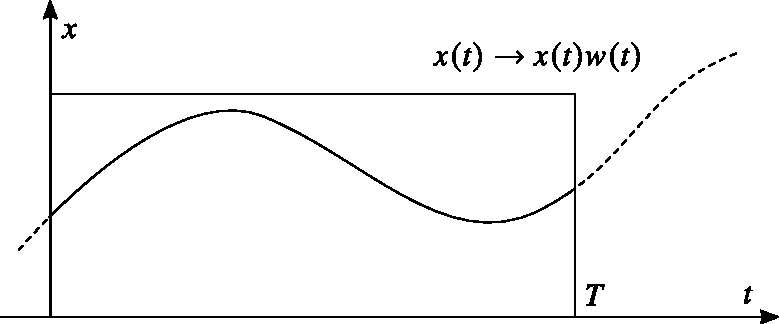
\includegraphics[width=0.8\textwidth]{window.pdf}
    \end{figure}
    \begin{align*}
        \mathcal{F}\left[x(t)w(t)\right] &= \int_{-\infty}^{+\infty} x(t)w(t) \e{-\j\omega t} \dif t \\
        &= \int_{0}^{T} x(t)w(t) \e{-\j\omega t} \dif t 
        = \frac{1}{2\uppi} X(\j\omega) \ast W(\j\omega)
    \end{align*}
\end{frame}

\begin{frame}{频率泄漏 --- 有限时间的截断效应}
    窗函数的影响
    \begin{figure}
        \centering
        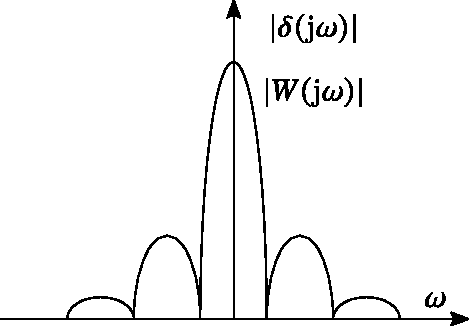
\includegraphics[width=0.5\textwidth]{window-function.pdf}
    \end{figure}
    \begin{itemize}
        \item 主瓣宽度:频率分辨率
        \item 旁瓣高度:频率泄漏
    \end{itemize}
\end{frame}


\begin{frame}{频谱混叠 --- 连续信号的采样失真}
    \begin{figure}
        \centering
        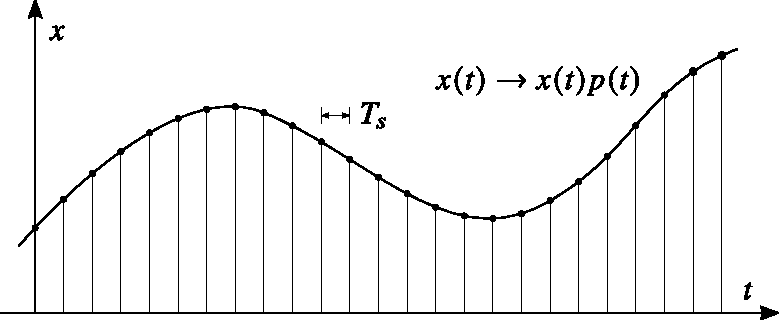
\includegraphics[width=0.8\textwidth]{sample.pdf}
    \end{figure}
    \begin{align*}
        \mathcal{F}\left[x(t)p(t)\right] &= \int_{-\infty}^{+\infty} x(t) \left(\sum_{n=-\infty}^{+\infty} \delta \left(t-nT_s\right)\right) \e{-\j\omega t} \dif t \\
        &= \frac{1}{2\uppi} X(\j\omega) \ast P(\j\omega)
        % \left( \frac{2 \uppi}{T_s} \sum_{k=-\infty}^{+\infty} \delta \left( \omega - n \frac{2 \uppi}{T_s}\right) \right)
        = \frac{1}{T_s} \sum_{k=-\infty}^{+\infty} X(\j\omega - \j k \omega_s)
    \end{align*}
\end{frame}


\begin{frame}{频谱混叠 --- 连续信号的采样失真}
    \begin{columns}
        \begin{column}{0.53\textwidth}
            \centering
            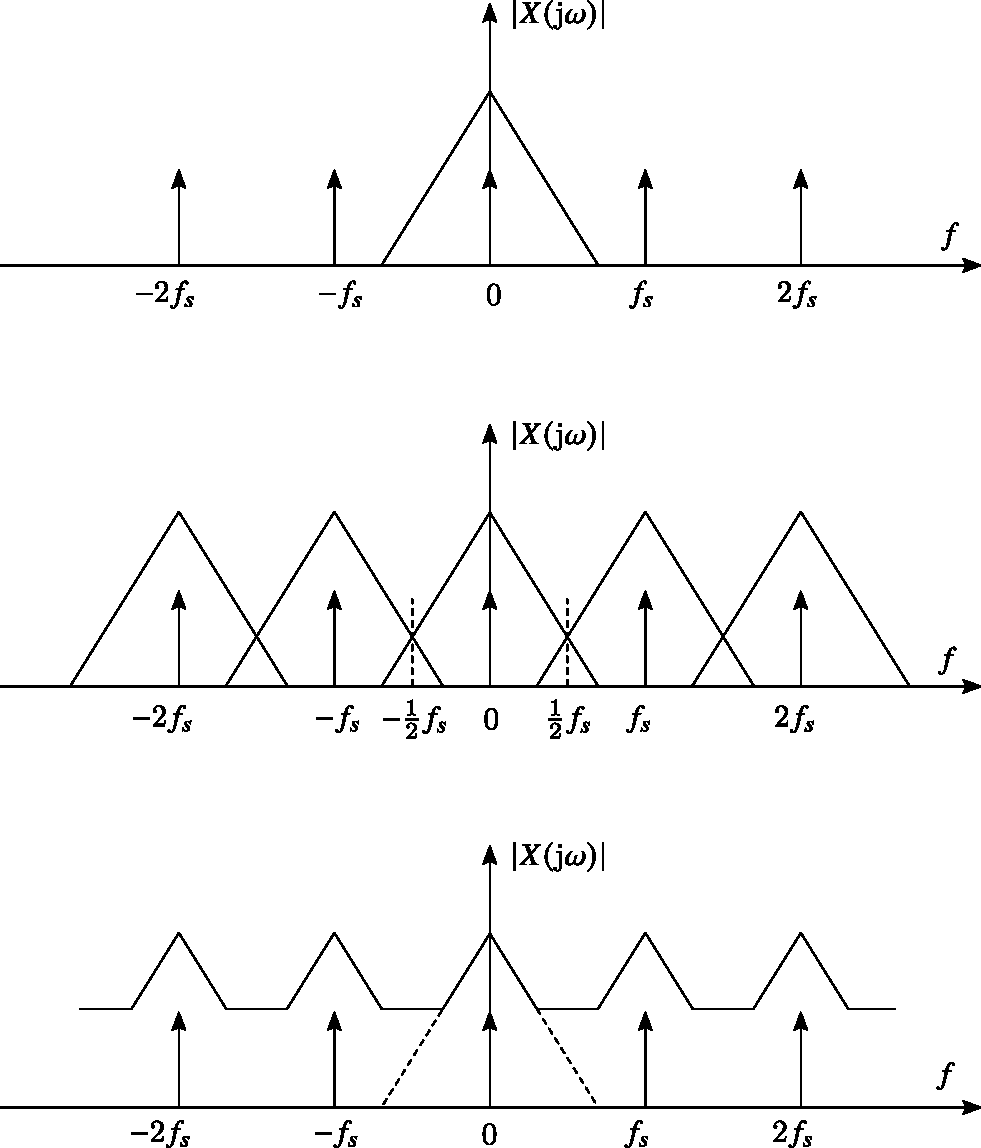
\includegraphics[width=\textwidth]{aliasing.pdf}
        \end{column}
        \begin{column}{0.4\textwidth}
            防止混叠的一般方法
            \begin{itemize}
                \item 抗混叠滤波器
                \item 提高采样率
            \end{itemize}
        \end{column}
    \end{columns}
\end{frame}


\begin{frame}{栅栏效应 --- 数字算法的离散本质}
    \begin{figure}
        \centering
        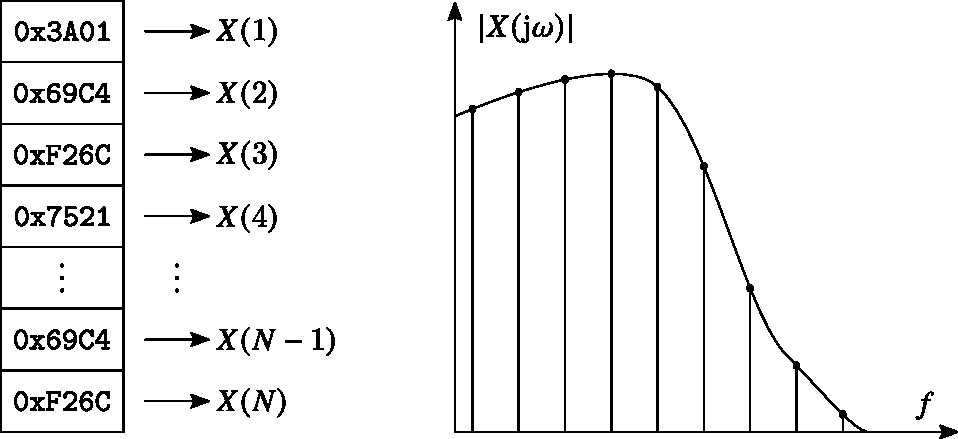
\includegraphics[width=0.8\textwidth]{discrete-data.pdf}
    \end{figure}
    减小栅栏效应的一般方法
    \begin{itemize}
        \item 增加采样点数
        \item 有效数据尾部补零
    \end{itemize}
\end{frame}


\begin{frame}{频率分辨率}
    频率分辨率:数据连续谱 $X(\j\omega)$ 中能够分辨的最小频率间隔

    计算分辨率:DFT算法所引入的频率间隔(栅栏效应)
    \begin{figure}
        \centering
        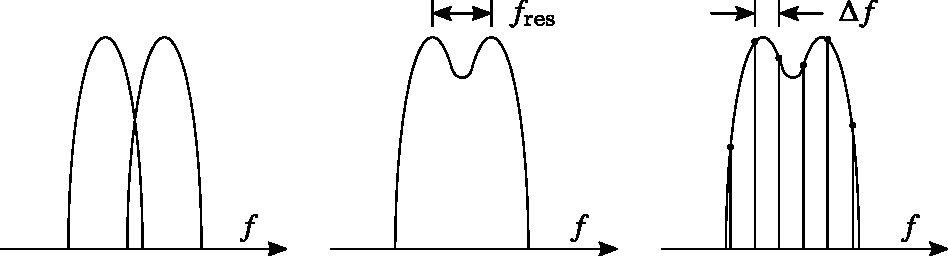
\includegraphics[width=\textwidth]{freqs-resolution.pdf}
    \end{figure}
    \begin{align*}
        f_{\rm res} = \frac{1}{T} \qquad \Delta f = \frac{f_s}{N}
    \end{align*}
    \footnote{程佩清. 数字信号处理. 第四版. 清华大学出版社. 2013. 185--189.}
\end{frame}

% =========================  第二节  =========================
\section{算法实现}
\begin{frame}{周期图法}
    \begin{columns}
        \begin{column}{0.6\textwidth}
            
        \end{column}
        \begin{column}{0.6\textwidth}
            
        \end{column}
    \end{columns}
    \small
    \texttt{[pxx,f] = periodogram(data,window,nfft,fs,'onesided');}
\end{frame}

\begin{frame}{Welch法}
    \small
    \texttt{[pxx,f] = pwelch(data,window,noverlap,nfft,fs,'onesided');}
\end{frame}

\begin{frame}{LPSD}
    \small
    \texttt{[pxx,f] = iLPSD(data,fs);}
    \footnote{M. Tröbs, G. Heinzel. Improved Spectrum Estimation from Digitized Time Series on a Logarithmic Frequency Axis. Measurement. 2006.
    }
\end{frame}


% =========================  第三节  =========================
\section{实际应用}
\begin{frame}{功率谱估计实际应用}
    \begin{itemize}
        \item 信号检测
        \item 噪声本底
        \item 系统辨识
    \end{itemize}
    
    \hfill
\includegraphics[width=0.25\textwidth]{share-code.pdf} \\
    \hfill\href{https://github.com/iChunyu/signal-process-demo}{\scriptsize https://github.com/iChunyu/signal-process-demo}
    
\end{frame}

\begin{frame}[standout]
    \zihao{0} 谢\ 谢\ !
\end{frame}

\end{document}